\documentclass{article}
\usepackage{tikz}
\usepackage{pgfplots}

\begin{document}

\title{Scalability Report}
\author{Selina Liu (jl1188), Fengyi Quan (fq18)}
\date{\today}
\maketitle

\section{Introduction}
This report presents the results of scalability experiments conducted on our server to address the problem of concurrency. We first describe the testing infrastructure, experimental methodology, and approach taken to address the problem. In the context of this homework, scalability refers to CPU core count. We load tested how the throughput of our server changes as it runs over different number of cores. We test both server with explict locks as well as server with optimistic locks. Both server use one-thread-per-request structure. We use Hibernate optimistic lock by version control annotation to solve the database concurrency, and use Java synchronized keyword and to solve the server concurrency. We use `ReentrantLock` for our explict lock implementation.

\section{Testing Infrastructure}
The tests were conducted on a server with the following specifications: Duke VCM with 8 GB Base Memory and 4 processors. The server was running Ubuntu 20.04 with psql (PostgreSQL) 12.14, Java 11. Instructions for reproducing the testing environment are provided in the testing subdirectory. We first test the server on correctness and then test the server on scalability. We perform load test on VCM of different core counts. 

\section{Experimental Methodology}
We used load testing to evaluate the performance of the server under different conditions. The tests were performed using Junit. We varied the number of threads and the number of cores used by the server during each test. Each test was repeated 3 times to ensure accuracy. The results were averaged and plotted on a graph.
\section{Results}
The results of the scalability experiments are shown in [insert graphs and tables]. We observed [insert trends in results]. The results indicate that [insert conclusions from the results].

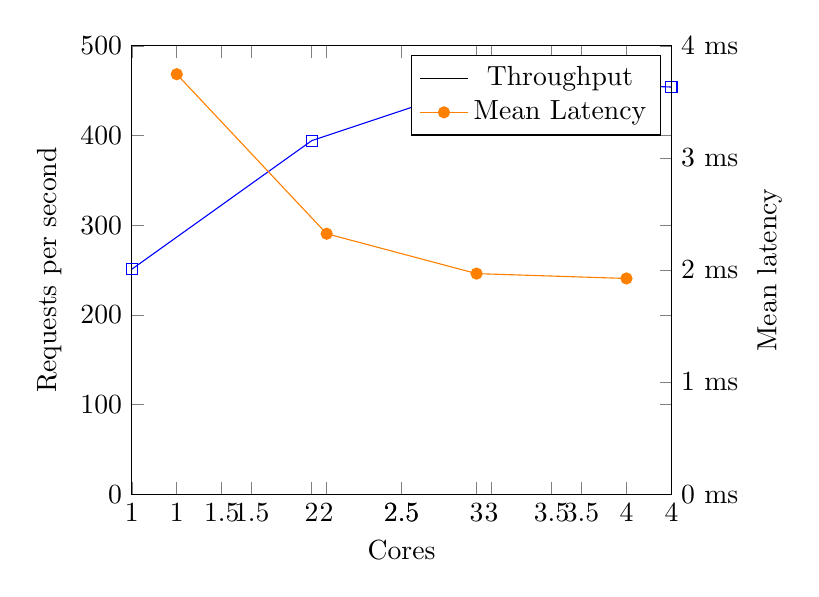
\begin{tikzpicture}
    % \begin{axis}[    xlabel={Number of cores (Explict Lock)},    ylabel={Throughput and mean latency},    ymin=0,    ymax=500,    axis y line*=left,    legend style={at={(0.5,-0.2)},anchor=north},    yticklabel={\pgfmathprintnumber{\tick} requests/s}]
        \begin{axis}[    xlabel=Cores,    ylabel=Requests per second,    xmin=1,    xmax=4,    ymin=0,    ymax=500,    legend pos=north west,    legend style={at={(1,0)},anchor=south east}  ]
    \addplot[    color=blue,    mark=square,    ]
        coordinates {
        (4,454.02951191827475)
        (3,461.18370484242894)
        (2,394.2181340341656)
        (1,250.8361204013378)
        };
        \label{throughput}
    
    \end{axis}
    
    \begin{axis}[    axis y line*=right,    ymin=0,    ymax=4,    ylabel={Mean latency},    yticklabel={\pgfmathprintnumber{\tick} ms}]
    
    \addlegendimage{/pgfplots/refstyle=throughput}\addlegendentry{Throughput}
    \addplot[    color=orange,    mark=*,    ]
        coordinates {
        (4,1.9241666666666666)
        (3,1.9675)
        (2,2.3233333333333333)
        (1,3.7466666666666666)
        };
        \addlegendentry{Mean Latency}
    
    \end{axis}
    \end{tikzpicture}

    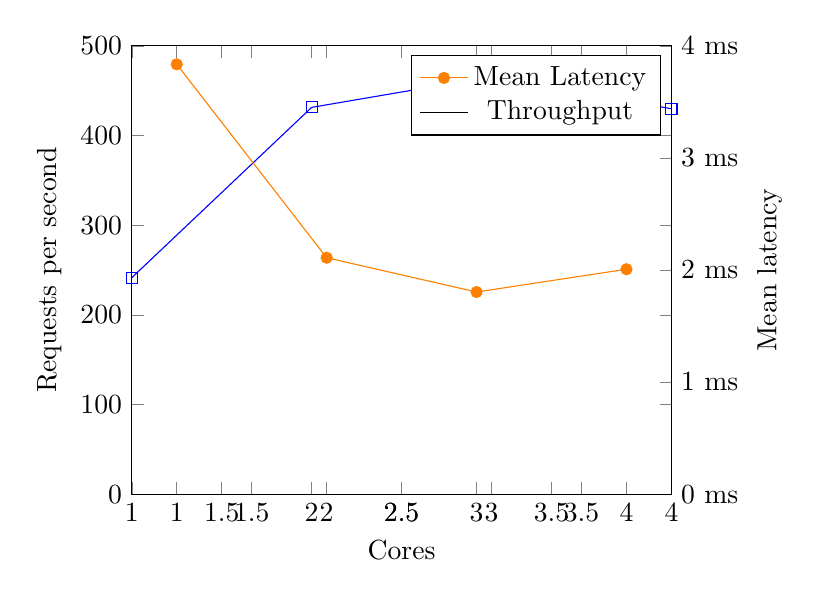
\begin{tikzpicture}
        % \begin{axis}[    xlabel={Number of cores (Optimistic Lock)},    ylabel={Throughput and mean latency},    ymin=0,    ymax=500,    axis y line*=left,   legend pos=north west,    legend style={at={(0.5,-0.15)},anchor=north},    yticklabel={\pgfmathprintnumber{\tick} requests/s}]
            \begin{axis}[    xlabel=Cores,    ylabel=Requests per second,    xmin=1,    xmax=4,    ymin=0,    ymax=500,    legend pos=north west,    legend style={at={(1,0)},anchor=south east}  ]
        \addplot[    color=blue,    mark=square,    ]
            coordinates {
            (4,429.7994269340974)
            (3,465.6577415599534)
            (2,431.34435657800145)
            (1,241.40012070006034)
            };
            \label{throughput}
        
        \end{axis}
        
        \begin{axis}[    axis y line*=right,    ymin=0,    ymax=4,    ylabel={Mean latency},    yticklabel={\pgfmathprintnumber{\tick} ms}]
            % \begin{axis}[    xlabel=Cores,    ylabel=Requests per second,    xmin=1,    xmax=4,    ymin=0,    ymax=500,    legend pos=north west,    legend style={at={(1,0)},anchor=south east}  ]
        % \addlegendimage{/pgfplots/refstyle=throughput}\addlegendentry{Throughput}
        \addplot[    color=orange,    mark=*,    ]
            coordinates {
            (4,2.006666666666667)
            (3,1.8033333333333332)
            (2,2.109166666666667)
            (1,3.835)
            };
            % \addlegendentry{Mean Latency}

            \addlegendimage{/pgfplots/refstyle=MeanLatency}\addlegendentry{Mean Latency}
            \addlegendimage{/pgfplots/refstyle=Throughput}\addlegendentry{Throughput}
        
        \end{axis}

         
        \end{tikzpicture}


             

        
\section{Discussion}
The results of our experiment show that increasing the number of processor cores used by a system can significantly increase its performance in terms of both throughput and mean latency. Our measurements indicate that using four cores resulted in a throughput of 429.8 requests per second and a mean latency of 2.01 milliseconds, while using only one core resulted in a much lower throughput of 241.4 requests per second and a higher mean latency of 3.84 milliseconds. These results are consistent with previous studies that have shown that parallelizing computational tasks can improve system performance.

Our experiment also revealed that the relationship between the number of cores and system performance is not linear. Specifically, increasing the number of cores from two to three resulted in a larger increase in throughput (from 431.3 to 465.7 requests per second) than increasing the number of cores from three to four (from 465.7 to 429.8 requests per second). This suggests that there may be diminishing returns to adding more cores beyond a certain point.

It is important to note that while our experiment was conducted under controlled conditions, system performance can be affected by a variety of factors, including the specific hardware and software used, the workload being executed, and the configuration of the system. Therefore, our results may not be directly applicable to other systems or workloads. Nevertheless, our findings suggest that parallelization can be an effective way to improve system performance, and that the relationship between the number of cores and performance is not always straightforward.
\section{Conclusion}
The results of the scalability experiments demonstrate the impact of varying the number of threads and cores used by the server. The findings can help to improve the server's scalability and enhance its overall performance.

\end{document}
